\begin{definicja}[Algorytm]\label{def:algorytm}
Zbiór jednoznacznie określonych reguł lub zadań obliczeniowych prowadzących w skończonej ilości kroków do rozwiązania pewnego problemu \cite{IEEE}.
\end{definicja}


Określone w ten sposób zadania obliczeniowe są z reguły względem siebie niezależne. Pewne z zadań mogą być wykonywane równolegle, inne muszą być wykonywane sekwencyjnie, jedno po drugim. Wobec tego algorytm może być określony częściowo równolegle, częściowo sekwencyjnie.


Podstawowymi elemetami określającymi dowolny algorytm są:
\begin{enumerate}
\item zadania do wykoniania,
\item zależności pomiędzy zadaniami polegające na określeniu czy 
dane wyjściowe któregoś z zadań nie są danymi wejściowymi dla innego zadania,
\item zbiór danych wejściowych wymaganych przez algorytm,
\item zbiór danych wyjściowych otrzymywanych po wykonania algorytmu.
\end{enumerate}

%Na podstawie niezależności zadań obliczeniowych algorytmy możemy %podzielić na pięć klas \cite{APC2011}:
%\begin{enumerate}
%\item Algorytmy szeregowe
%\item Algorytmy równoległe
%\item Algorytmy szeregowo--równoległe (SPA, Serial--Parallel %Algorithms)
%\item Algorytmy nieszeregowo--równoległe (NSPA, Nonserial--%Parallel Algorithms)
%\item Algorytmy regularno-iteracyjne (RIA, Regular--Iterative %Algorithms)
%\end{enumerate}

\begin{definicja}[Algorytm sekwencyjny]\label{def:algorytm_sekwencyjny}
\textbf{Algorytm sekwencyjny} (rys.  \ref{fig:sequential}) jest ciągiem dokładnie sprecyzowanych zadań obliczeniowych \(T_i,\, i\in\mathbb{N}\) rozwiązujących dany problem, tj. wyznaczających dane wyjściowe na podstawie danych wejściowych. Zakłada się, że w algorytmie sekwencyjnym zadania wykonywane są przez jeden procesor.

\end{definicja}

\begin{figure}[h]
\centering
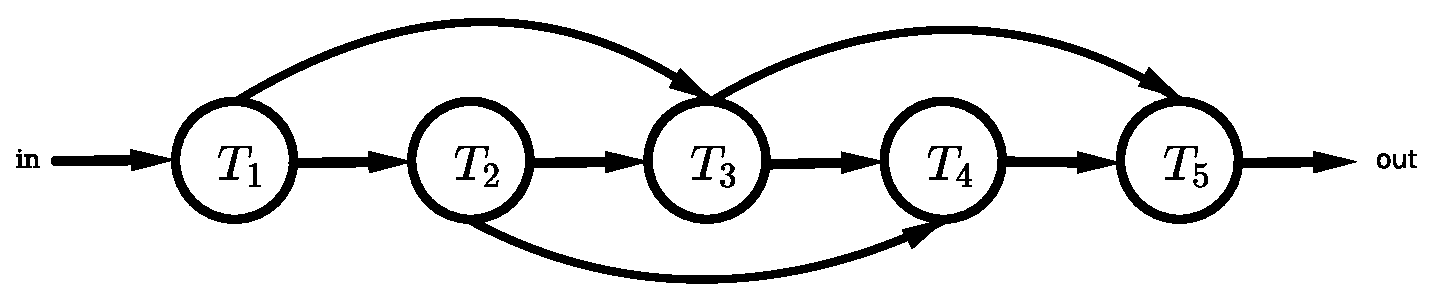
\includegraphics[width=14cm]{images/Rys2.eps}
\caption{Algorytm sekwencyjny}
\label{fig:sequential}
\end{figure}

W celu rozwiązania problemu za pomocą większej liczby procesorów należy go zdekomponować na podproblemy, które mogą być rozwiązane równolegle. Każdy z podproblemów rozwiązywany jest przez odrębny algorytm będący składową algorytmu równoległego.


\begin{definicja}[Równoległość]\label{def:rownoleglosc}
\textbf{Równoległość} w odniesieniu do oprogramowania jest to symultaniczny transfer, występowanie albo przetwarzanie poszczególnych części pewnej całości, takich jak bity składające się na znak albo znaki pewnego słowa, używając osobnych urządzeń dla ich różnych części \cite{IEEE}.
\end{definicja}


\begin{definicja}[Algorytm równoległy]\label{def:algorytm_rownolegly}
\textbf{Algorytmem równoległym} (rys. \ref{fig:parallel}) nazywamy każdy algorytm, w którym spośród określonych w nim zadań \(T_1\), \(T_2\), \(\dots\), \(T_n\) co najmniej dwa zadania \(T_i\), \(T_j\), \(i\neq j\) dzięki ich wzajemnej niezależności, mogą być wykonane równocześnie \cite{APC2011}.\\
\end{definicja}

\begin{figure}[h]
\centering
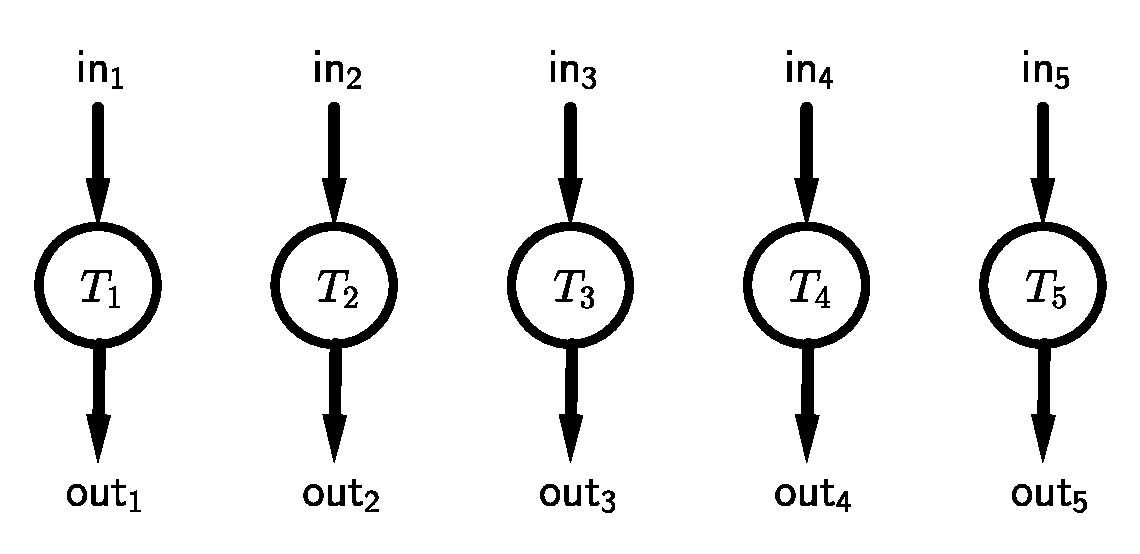
\includegraphics[width=10cm]{images/Rys1.eps}
\caption{Algorytm równoległy}
\label{fig:parallel}
\end{figure}

\begin{przyklad}
Prostym przykładem algorytmu równoległego jest serwer sieciowy, który każde zapytanie przychodzące przetwarza niezależnie od innych zapytań. Innym przykładem są wielozadaniowe systemy operacyjne radzące sobie z jednoczesną obsługą kilku uruchomionych programów.
\end{przyklad}

%
%\begin{definicja}[Algorytmy szeregowo--równoległe]
%
%\end{definicja}
%
%\begin{definicja}[Algorytmy nieszeregowo--równoległe]
%\end{definicja}
%
%\begin{definicja}[Algorytmy regularno--iteracyjne]
%Algorytmy tej klasy reprezentowane za pomocą grafów zależności wyrażają pewien pewien ustalny schemat postępowania.
%\end{definicja}